\chapter{Aufbau}
Abbildung \ref{aufbau} zeigt den physischen Aufbau des Projekts. Auf der einen Seite ist der Raspberry PI erkennbar. Auf der anderen Seite befindet sich ein Arduino UNO, welcher einen Datenlogger darstellen soll. Da zur Zeit der Entwicklung der explizit dafür vorgesehene Datenlogger nicht verfügbar war, wurden mittels eines Arduino UNO dessen Funktionalitäten nachgebaut. Der Arduino UNO zählt die ankommenden Impulse und summiert diese auf. Per Konsole werden die Werte an den Entwickler gegeben, sodass er testen kann, ob die gewünschte Anzahl von Impulsen angekommen ist. Im Betrieb soll jedoch ein richtiger Datenlogger zum Einsatz kommen.\\
Den Kern des Aufbaus bildet der Optokoppler vom Typ KB Knighbright KB 817. Der Optokoppler trennt die beiden Stromkreise galvanisch voneinander. Diese Trennung sichert den Raspberry PI gegen zu hohe Spannungen ab und verhindert somit seine Zerstörung. 
\begin{figure}[H]
 	\centering
 	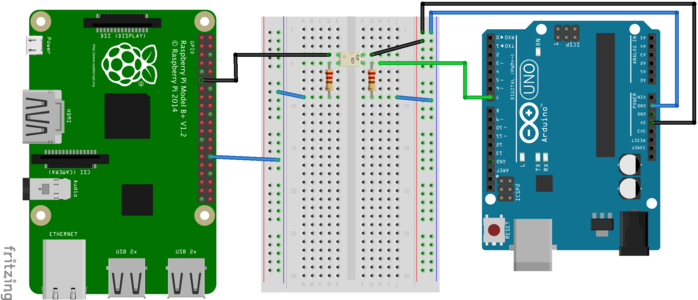
\includegraphics[width=0.8\textwidth]{bilder/aufbau.png}
 	\caption{Schematischer Aufbau}
	\label{aufbau}
\end{figure}
\noindent
Im eigentlichen Betrieb läuft der Simulator mit dem e.manager der Firma enerserve. Der e.manager erlaubt es Anlagen zu überwachen und deren Verbrauch zu messen. Dies geschieht über diverse Schnittstellen, darunter auch die S0-Schnittstelle. Da der e.manager mit einer Spannung von 12 Volt betrieben wird, muss dieser galvanisch vom Raspberry PI getrennt werden, da dieser mit 5 Volt betrieben wird. Dies geschieht mit dem bereits erwähnten Optokoppler. Abbildung \ref{emanager} zeigt den Aufbau mit dem Raspberry PI und dem e.manager.
 \begin{figure}[H]
 	\centering
 	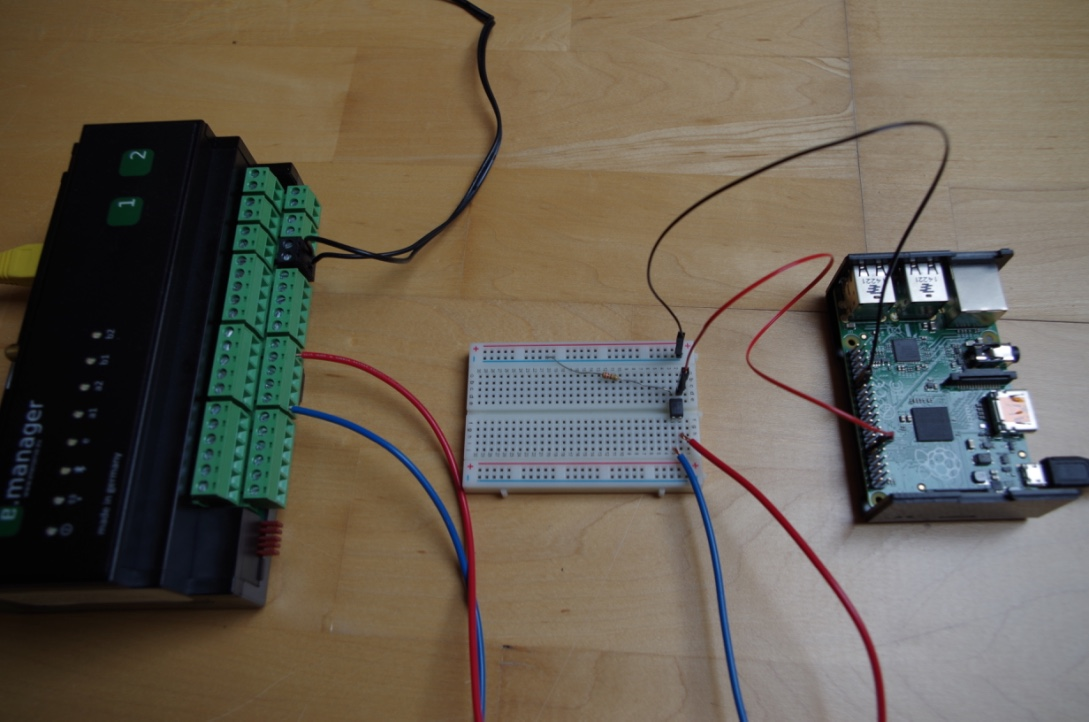
\includegraphics[width=0.8\textwidth]{bilder/aufbau.jpg}
 	\caption{Aufbau mit e.manager}
 	\label{emanager}
 \end{figure}
 \noindent
 Die ermittelten Daten des e.managers können über ein Webinterface abgerufen werden. Das Portal von enerserve (http://portal.enerserve.eu) erlaubt es dem Benutzer den Verlauf der einzelnen Geräte zu verfolgen. Neben einer Übersicht des aktuellen Verbrauchs, liefert das Webinterface auch historische Daten. Dabei wird zwischen Tages-, Monats- und Jahresansicht unterschieden. Weiterhin bietet das Interface eine Konfiguration der Anschlüsse.